%----------------------------------------------------------------------------------------
%	PACKAGES AND DOCUMENT CONFIGURATIONS
%----------------------------------------------------------------------------------------
\documentclass[11pt, a4]{article}
\usepackage{amsmath} % Required for some math elements
\usepackage{hyperref} 
\usepackage{xcolor}
\usepackage{lipsum} 
\usepackage{cite}
\usepackage{graphicx} % Required for the inclusion of images
\usepackage{algorithmic}
\usepackage{array}
\usepackage{bookmark}
\usepackage{listings}
\usepackage{amssymb}
\usepackage{enumitem}
\usepackage[margin=24mm, paperheight=300mm]{geometry}
\usepackage[caption=false, font=footnotesize]{subfig}
\usepackage{multirow}

\newlist{steps}{enumerate}{1}
\setlist[steps, 1]{label = Step \arabic*:}

\hypersetup{ %color attributes of citation, link, etc.
    colorlinks=true,
    linkcolor=blue,
    filecolor=gray,      
    urlcolor=blue,
    citecolor=blue,
}

\newcommand{\matlab}{\textsc{Matlab }} %very important and totally necessary addition

\newcommand\Item[1][]{%
  \ifx\relax#1\relax  \item \else \item[#1] \fi
  \abovedisplayskip=0pt\abovedisplayshortskip=0pt~\vspace*{-\baselineskip}}
  %----------------------------------------------------------------------------------------
%	DOCUMENT INFORMATION
%----------------------------------------------------------------------------------------
 
\title{ECEN303 : Analogue \\ Design Exercise 2020}
\author{Daniel Eisen : 300447549}
\date{\today}

\begin{document}
\maketitle
\tableofcontents
%----------------------------------------------------------------------------------------
%	DOCUMENT CONTENT
%----------------------------------------------------------------------------------------
\section{Introduction}
This report outlines the design of a duel output (mains) AD/DC power supply.
It must meet the following specifications:
\begin{itemize}
        \item Accept NZ mains AC input
        \item 5V, 3A output with a $V_out$ ripple $\le$0.5\%
        \item 2.5V, 100mA output with a $V_out$ ripple $\le$0.1\%
        \item Total cost under US\$30
\end{itemize}

The basic overview of this topology is a AD/DC fly-back stage from mains to an intermediate voltage and 2 buck DC/DC converters to give the final output supplies.

This was achieved primarily with the use of TI-WEBENCH Power Designer\cite{tibad} for design and simulation/evaluation. 

\section{AC/DC}
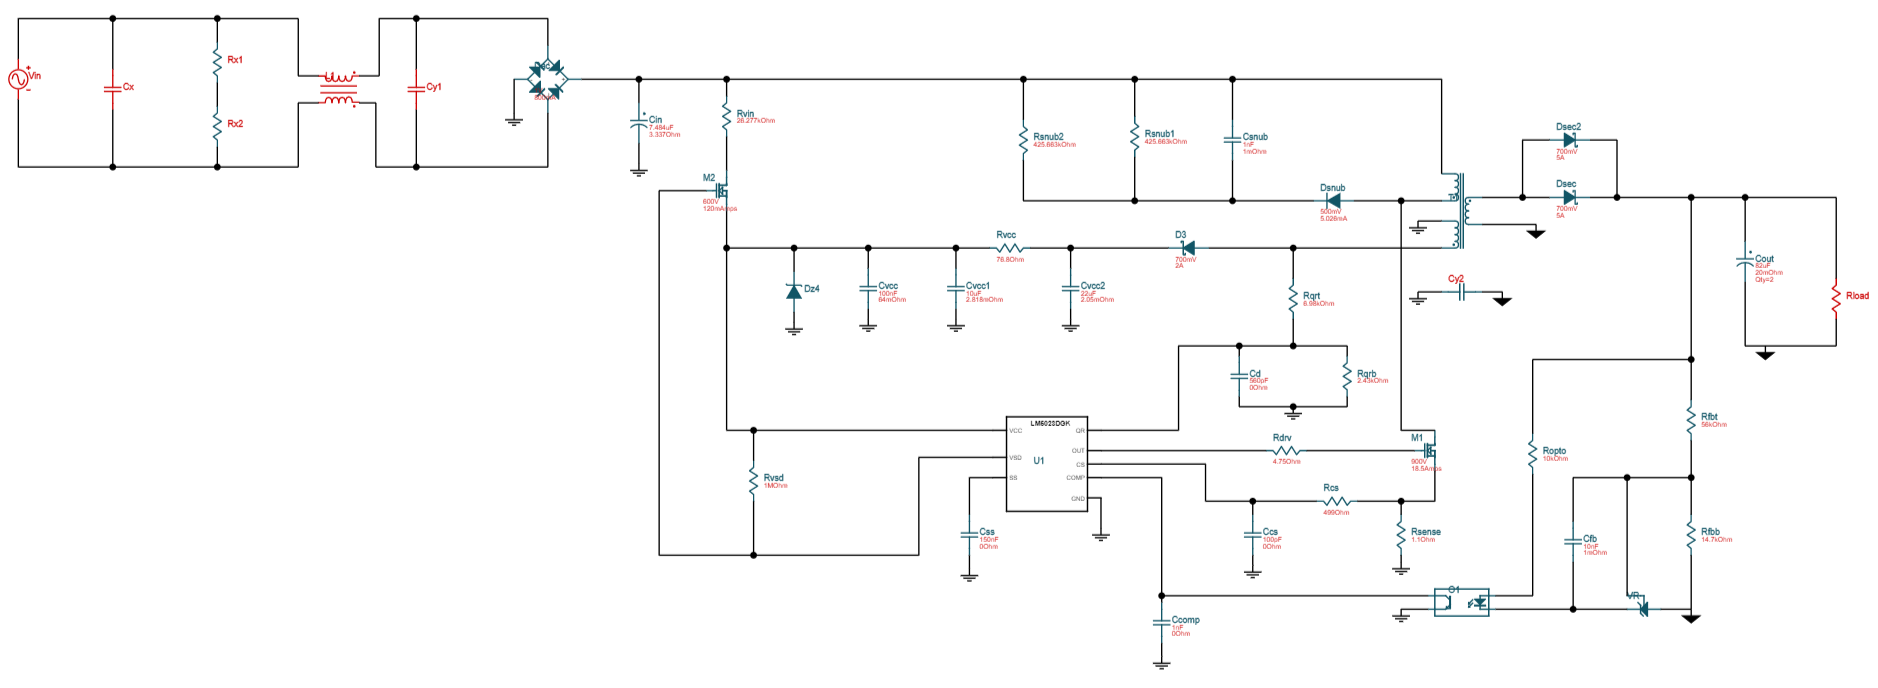
\includegraphics[width=\textwidth]{img/acdc.png}
\begin{center}
        Figure 1.
\end{center}
\subsection{Design}
This First input stage of the PSU is an AC/DC fly-back converter. It was designed to take standard New Zealand mains as an input; this is 230V with a $\pm6\%$ tolerance\cite{mains}, ie min/max of 216/244.

It outputs a intermediate voltage (further buck conversion stages) at a nominal 12V, 2A max current to facilitate the current draw from both output stages.

It includes an input stage EMI filter (see Figure 1), that allows the 50Hz AC through but has a high impedance to any higher frequency.

As this design could not be simulated, it is assumed to operate at its noted nominal efficiency with ideal output ripple.
\subsection{Results}
\begin{center}
        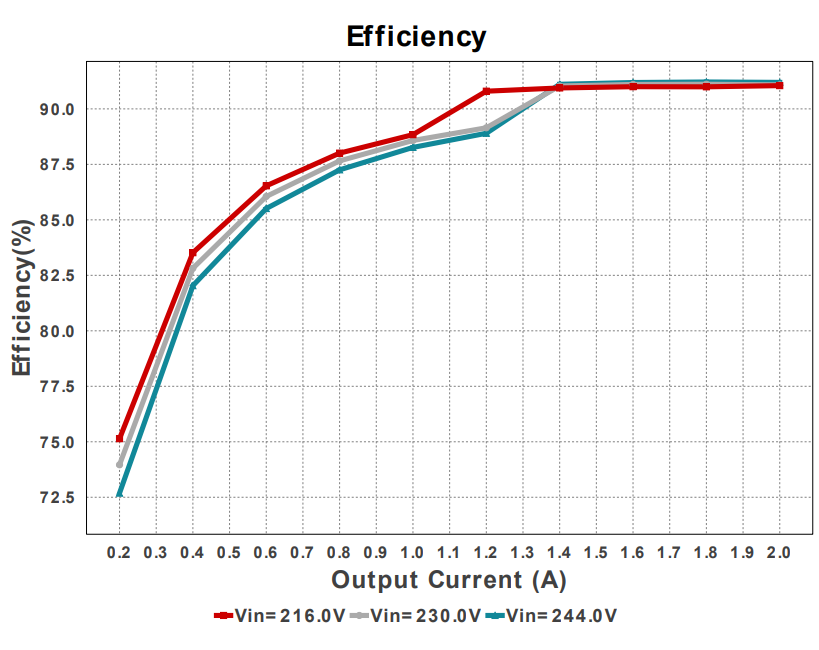
\includegraphics[width=0.4\textwidth]{img/acdc_eff.png} \\
        Figure 2.
\end{center}

An efficiency simulation was run. The design is shown to have a nominal operation efficiency of 91\%, with characteristic curve shown in Figure 2.

\section{DC/DC 5V 3A}
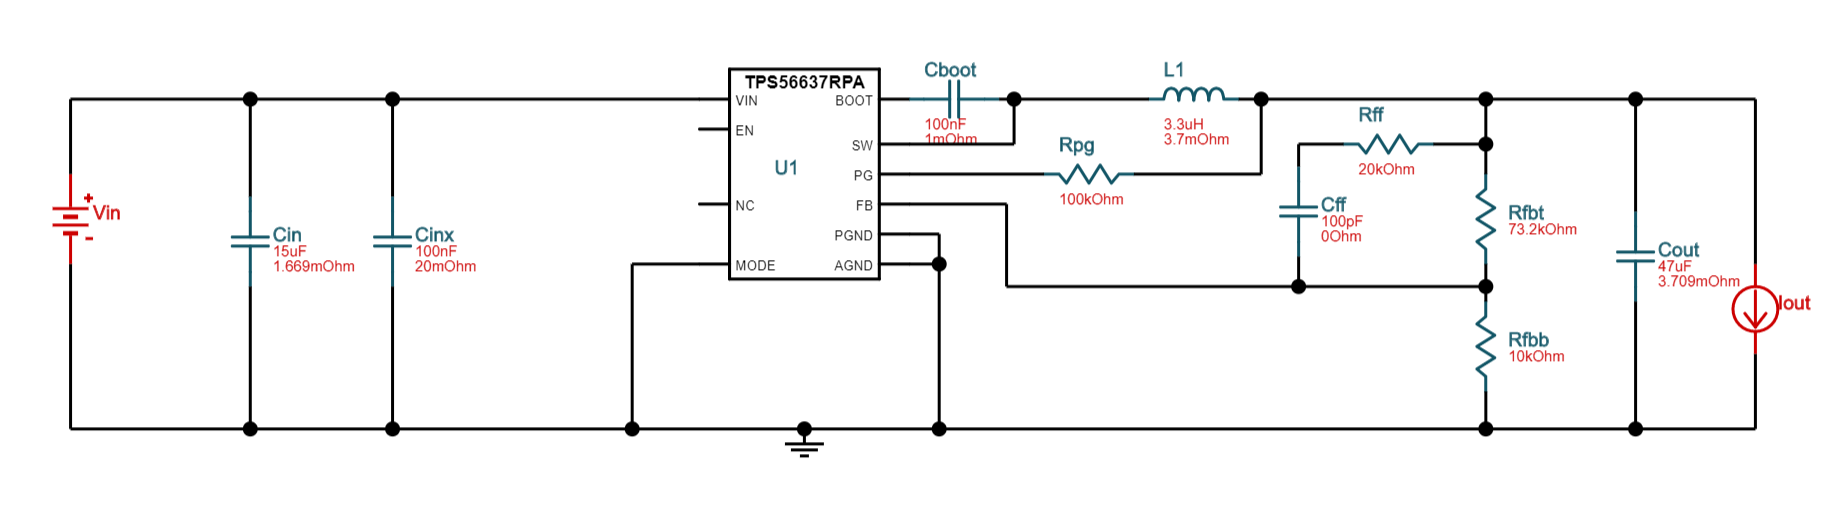
\includegraphics[width=0.9\textwidth]{img/dcdc5V.png}
\begin{center}
        Figure 3.
\end{center}
\subsection{Design}
This first output stage is specified to supply 5V at 3A, this was achieved with the above buck converter design. Chosen for it's high efficiency, and low footprint/complexity.

It was required to meet the ripple tolerance outlined above and take the first stage intermediate output as the nominal input voltage.
\subsection{Results}
\begin{center}
        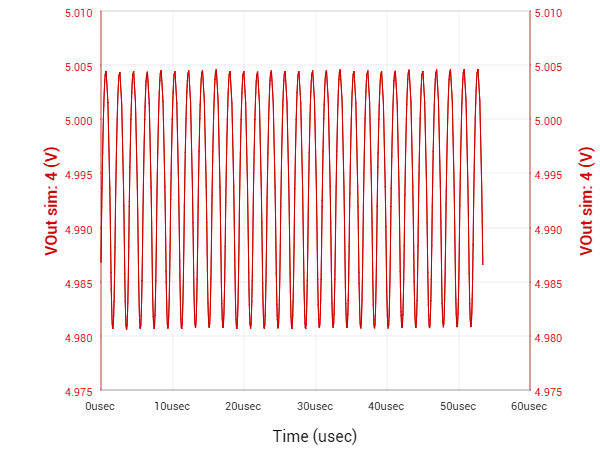
\includegraphics[width=0.4\textwidth]{img/5v_ripple.png}
        Figure 4.
\end{center}
A steady state analysis simulation was run to evaluate its output ripple performance. The Results of which are seen in figure 4.
This design evaluated to a Vout p-p of 23.667 mV, ie a 0.47334\% ripple. This is within spec (0.5)
\begin{center}
        \includegraphics[width=0.4\textwidth]{img/5V_eff.png}
        Figure 5.
\end{center}
An efficiency simulation was run. The design is shown to have a nominal operation efficiency of 94.1\%, with characteristic curve shown in Figure 5.


\section{DC/DC 2.5V 100mA}
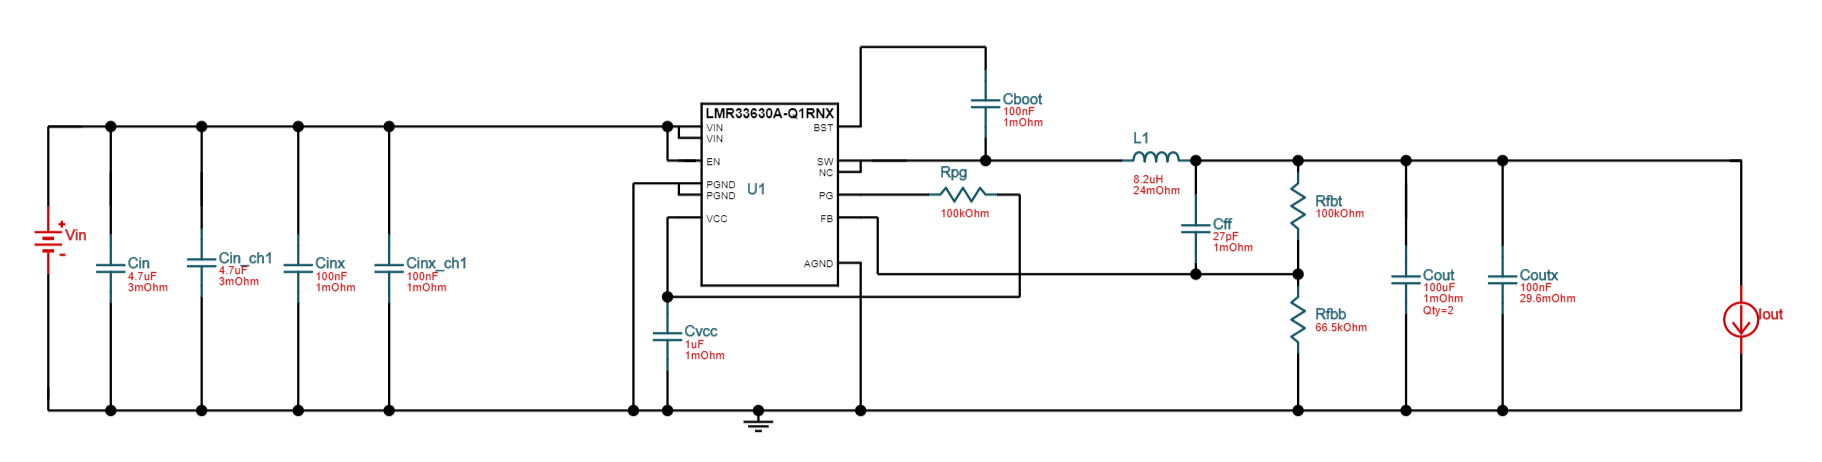
\includegraphics[width=0.9\textwidth]{img/dcdc2V5.png}
\begin{center}
        Figure 6.
\end{center}
\subsection{Design}
This next stage is specified to supply 2.5V at 100mA, this was achieved with the above buck converter design. Chosen for it's high efficiency, and low footprint/complexity. In this case do to low expected power draw its efficiency will not overly impact total design, however it was still optimised to that.

It was required to meet the ripple tolerance outlined above and also take the first stage intermediate output as the nominal input voltage.
\subsection{Results}

\begin{center}
        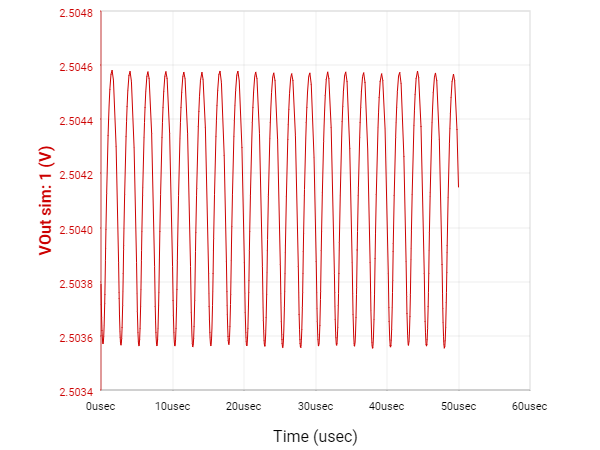
\includegraphics[width=0.4\textwidth]{img/2-5-ripple.png}
        Figure 7.
\end{center}
A steady state analysis simulation was run to evaluate its output ripple performance. The Results of which are seen in figure 7.
This design evaluated to a Vout p-p of 1.502 mV mV, ie a 0.06008\% ripple. This is within spec (0.1)
\begin{center}
        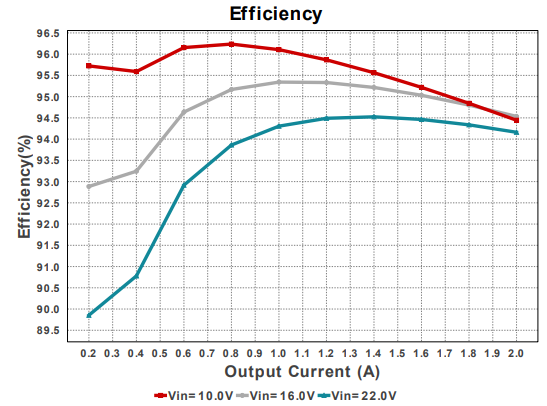
\includegraphics[width=0.4\textwidth]{img/2-5V_eff.png}
        Figure 8.
\end{center}
An efficiency simulation was run. The design is shown to have a nominal operation efficiency of 94.2\%, with characteristic curve shown in Figure 8.


\section{Final Design and Protection}
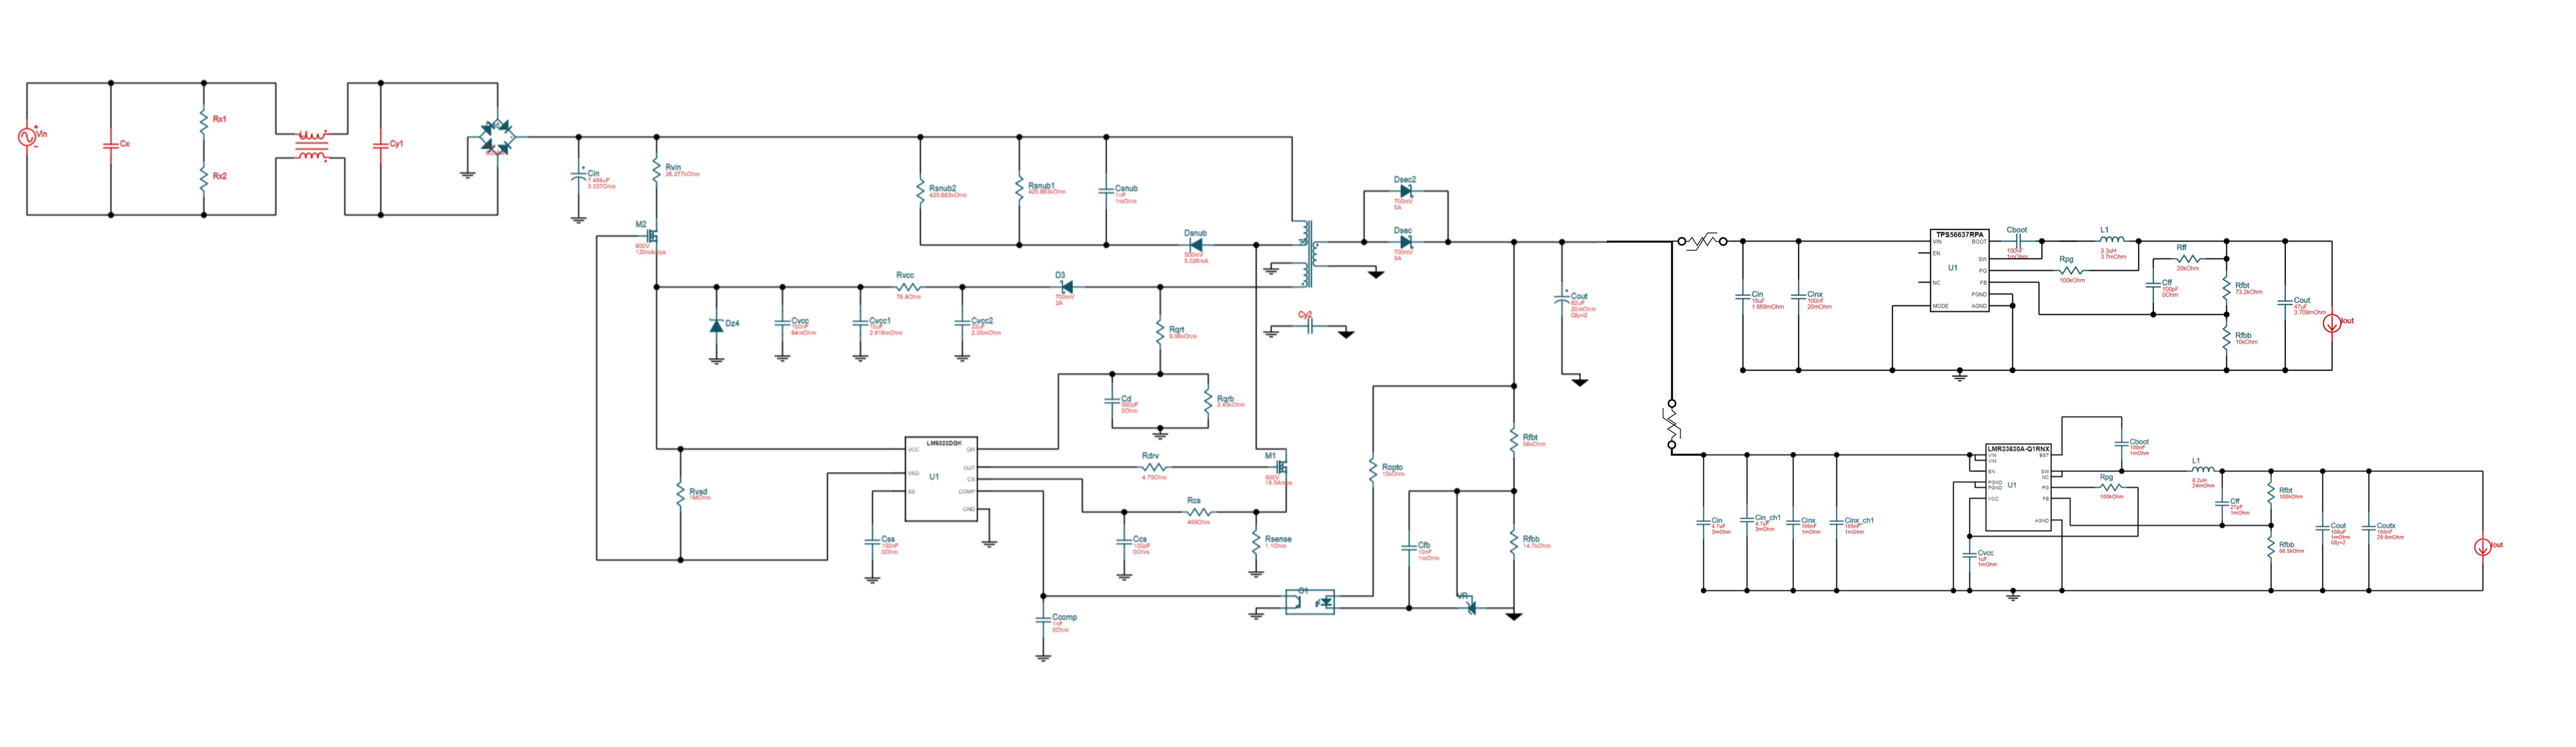
\includegraphics[width=0.9\textwidth]{img/full.png}
\begin{center}
        Figure 9.
\end{center}
\subsection{Design}
To complete the design the 3 above stage must be combined, and added over-current protection included for each stage. This is achieved with resettable poly-fuse, with a trip current of 1.5A. The designs themselves are feedback based so this is the only required addition.
\subsection{Results}
Total Efficiency: \\
Calculate the power out of each output buck stage:
\begin{align*}
    P_{o-5V}   &= 5V \cdot 3A\\
                 &= 15W\\\\
    P_{o-2.5V} &= 2.5V \cdot 100mA\\
                 &= 0.25W\\\\
\end{align*}

Calculate the power into each output buck stage, to get power draw AC/DC stage:
\begin{align*}
    P_{i}      &= \frac{P_o}{\eta}\\
    P_{i-5V}   &= \frac{15W}{0.941}\\
                &= 15.940W\\\\
    P_{i-2.5V} &= \frac{0.25W}{0.942}\\
                &= 0.265W\\\\
    P_{i-5V} + P_{i-2.5V} &= 16.205W
\end{align*}

Power into the AC/DC stage:
\begin{align*}
    P_{i}      &= \frac{P_o}{\eta}\\
    P_{i-AC}   &= \frac{16.205}{0.91} \\
                &= 17.808W
\end{align*}

Now we calculate the overall efficiency:
\begin{align*}
    \eta &= \frac{P_o}{P_i} \\
         &= \frac{P_{o-5V}+ P_{o-2.5V}}{P_i} \\
         &= \frac{15.25}{17.808} \\
         &= 86\%
\end{align*}

In total, the PSU has a final overall efficiency of 86\%, both stages meet their ripple requirements and the total BOM cost (see Appendix) is under US\$30, coming to US\%18.22

\newpage
\section*{Appendix}
\subsection*{AC/DC Parameters}
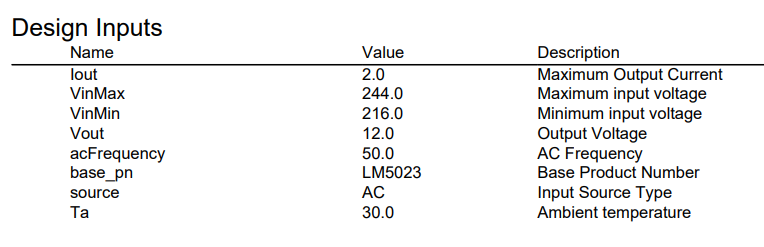
\includegraphics[width=\textwidth]{img/acdc_param.png}
\subsection*{5V DC/DC Parameters}
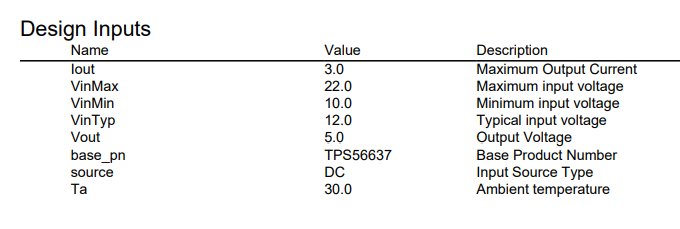
\includegraphics[width=\textwidth]{img/5v_param.png}
\subsection*{2.5V DC/DC Parameters}
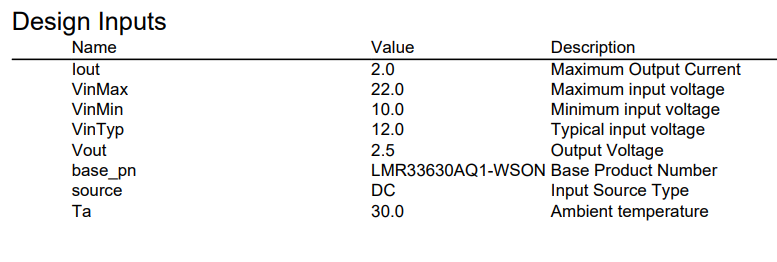
\includegraphics[width=\textwidth]{img/2-5V_param.png}
\newpage
\subsection*{AD/DC Transformer}
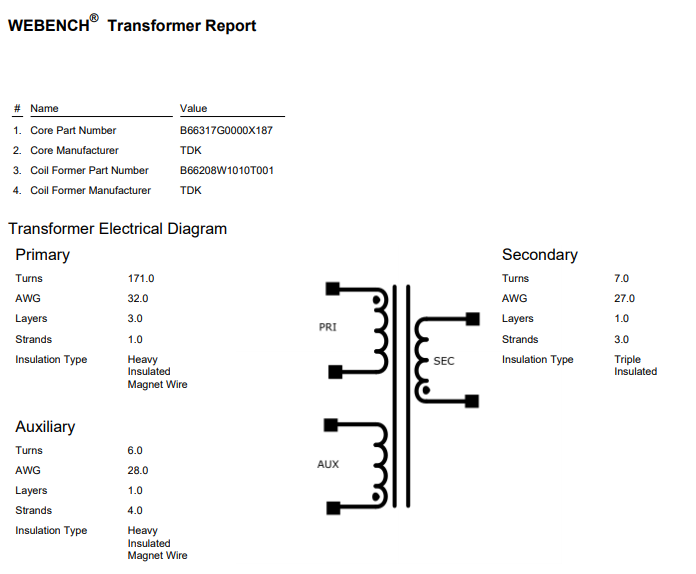
\includegraphics[width=\textwidth]{img/acdc_transformer.png}
\subsubsection*{BOM}
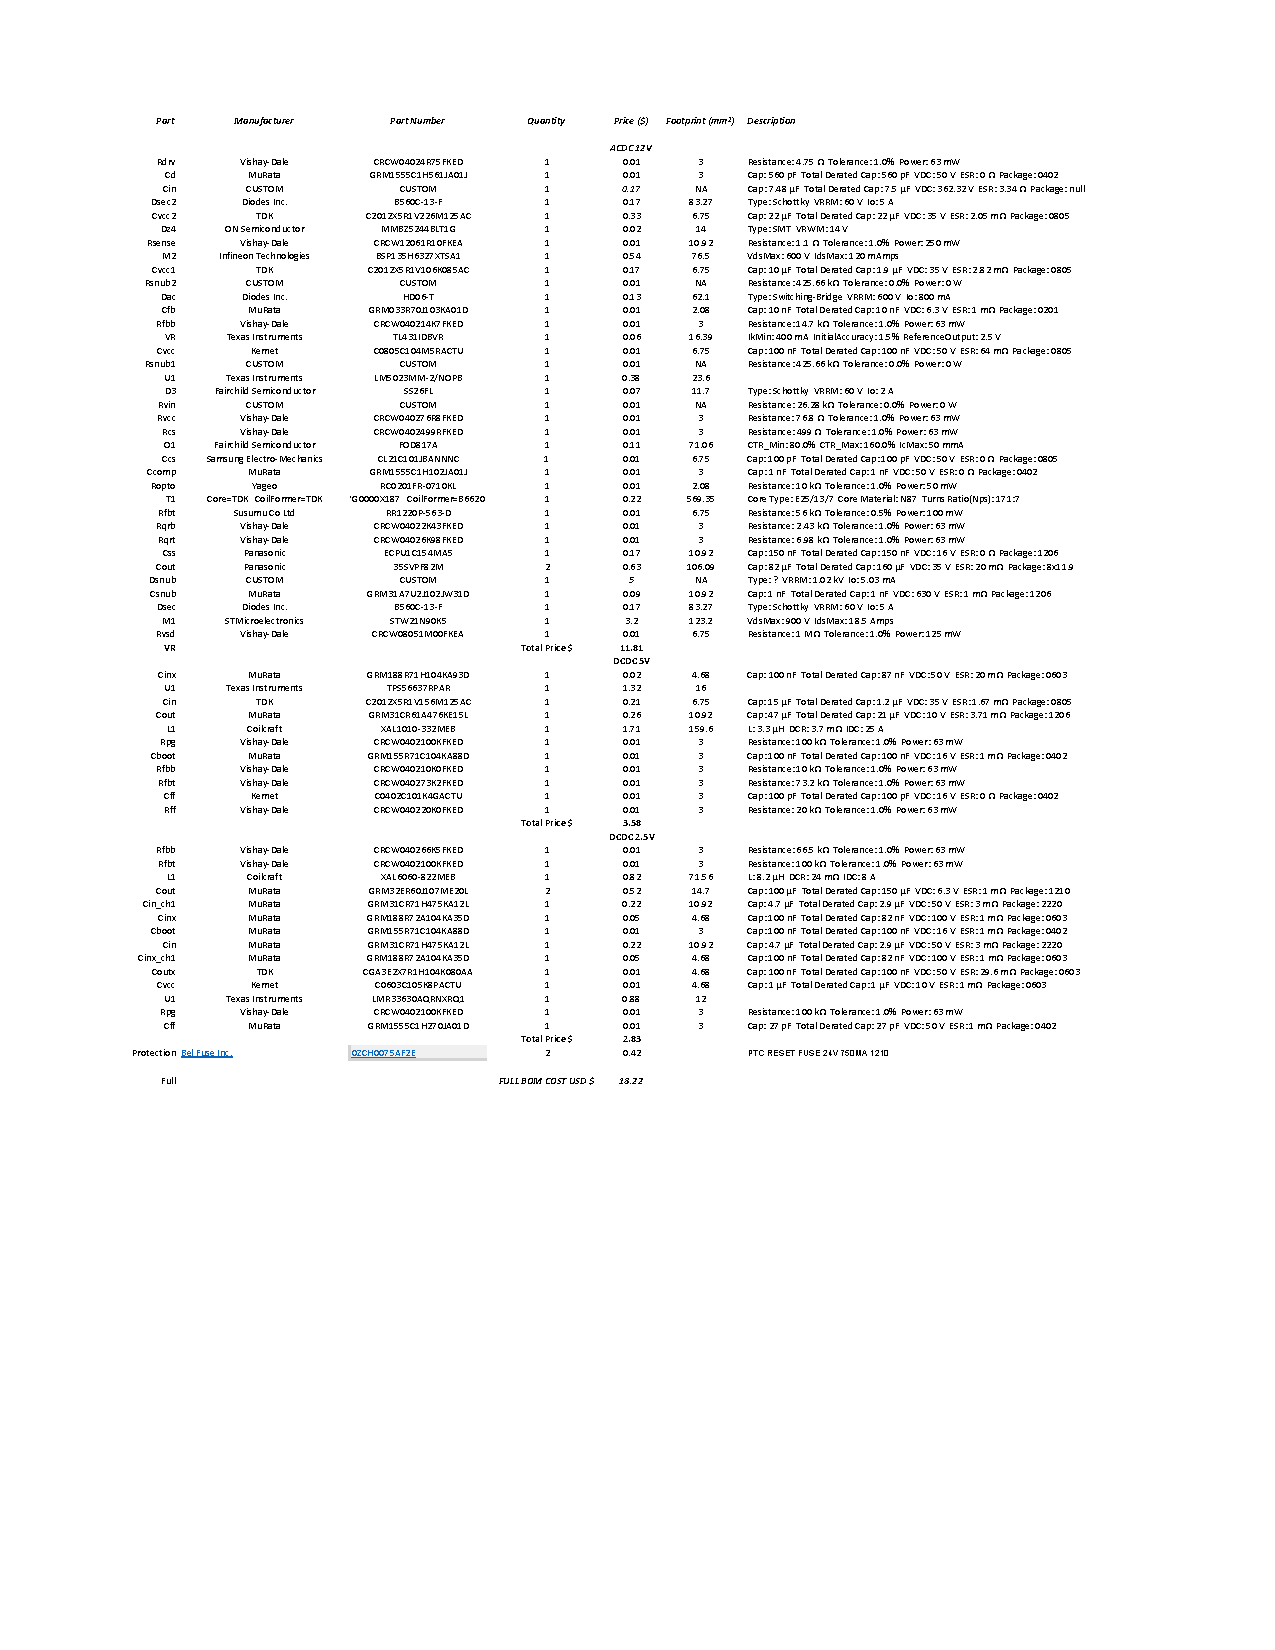
\includegraphics[width=\textwidth]{BOM.pdf}

\bibliography{ref}
\bibliographystyle{IEEEtran}
\end{document}